\section{Results}
\label{sec:results}

\subsection{The activity audit changes the reference calculation}

The apparent discrepancy in FY2023--24 cement activity results from an incorrect period
assignment. PBS QIM and the SBP
fiscal series both report \SI{39.566}{\mega\tonne}; the former
\SI{48.011}{\mega\tonne} statistic is the FY2021--22 value. The corrected reference therefore
contains \SI{29.6745}{\mega\tonne} of clinker at a 0.75 fraction. Adding
\SI{3.792074}{\mega\tonne} of exports and subtracting
\SI{0.026131}{\mega\tonne} of imports gives \SI{33.440443}{\mega\tonne} of inferred domestic
clinker production (Table~\ref{tab:balance}). At \SI{0.52}{\tonne\per\tonne}, process
emissions on that inferred route are \SI{17.389030}{\mega\tonne} \COtwo{}---the named
Tier~1 diagnostic. The reference does not use the inferred route: it takes the
\SI{41.953170}{\mega\tonne} of clinker the sixteen producers report and gives
\SI{21.815648}{\mega\tonne} \COtwo{} at the same factor.

\begin{table}[htbp]
\centering
\footnotesize
\begin{tabular}{@{}lrr@{}}
\toprule
\textbf{Clinker flow} & \textbf{Mt} & \textbf{Sign in inferred production} \\
\midrule
Clinker contained in cement & 29.674 & $+$ \\
Imports                     &  0.026 & $-$ \\
Exports                     &  3.792 & $+$ \\
Stock increase              &  0.000 & $+$ \\
\midrule
\textbf{Inferred domestic production} & \textbf{33.440} & \\
\bottomrule
\end{tabular}
\caption{FY2023--24 clinker balance. The zero stock row is explicit and unresolved.}
\label{tab:balance}
\end{table}

Using the correct FY2023--24 activity but omitting observed trade gives
\SI{15.430740}{\mega\tonne} \COtwo{}. Trade correction therefore adds 1.958 Mt, or 12.7\%,
and is a method correction rather than a valid structural alternative. The original
18.724 Mt result is retained only as a historical benchmark because it combines trade omission with the
misdated 48.011 Mt activity.

\subsection{Producer evidence against the two Tier~1 inferences}

All sixteen company filings sum to \SI{41.953170}{\mega\tonne} of actual clinker, equivalent
to \SI{21.815648}{\mega\tonne} \COtwo{} at the common factor---the reference activity. This
observed census is 125.5\% of the 0.75 Tier~1 inference and 101.4\% of the 0.95
inference---a near-identity that partly reflects the two constructions drawing on
overlapping reporting, and is therefore construction similarity as much as corroboration;
Fecto's quantity is read from its FY2025 annual report's comparative table
(Figure~\ref{fig:producers}). We use the reported census without extrapolation. If the company filings
and QIM cover the same producers and reporting period, and stock change is negligible, the
observed subset implies a diagnostic clinker fraction of 0.949. The low-clinker case is
therefore inconsistent with the company data unless the two sources differ in producer
coverage or reporting period, or unless clinker transfers and stock changes materially affect
the balance.

The company compilation constrains the national clinker balance but does not yet constitute a
complete Tier~2 activity dataset. A consistent set of opening and closing stocks, clinker
purchases, domestic sales, exports and clinker ground has not been reported. The unresolved
terms are documented without allocating the national residual among firms.

\begin{figure*}[htbp]
\centering
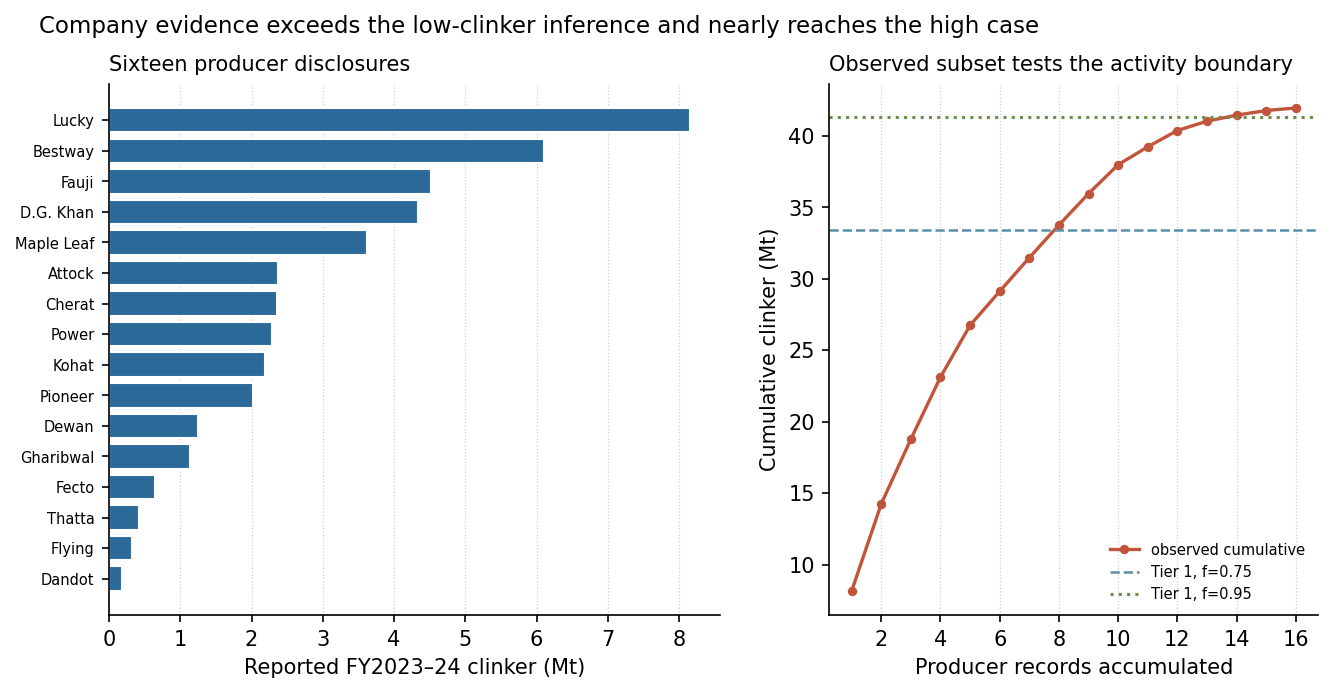
\includegraphics[width=0.98\textwidth]{ippu_producer_census.png}
\caption{Reported FY2023--24 clinker by producer (left) and the cumulative observed subset
against the two trade-corrected Tier~1 inferences (right). All sixteen census producers
report an exact quantity; Fecto's is the FY2024 comparative of its FY2025 annual report.}
\label{fig:producers}
\end{figure*}

\subsection{Valid cement models and conditional uncertainty}

With observed trade included in every current model, the structural range is
17.389--21.504 Mt \COtwo{} for clinker fractions of 0.75 and 0.95
(Figure~\ref{fig:cementevidence}); both ends of that range are priced against the
national total as named configurations in
\texttt{outputs/national\_configurations.csv}, and the observed census (21.816 Mt) sits
1.4\% above the high end. The reference Monte Carlo has a median of
\SI{21.809297}{\mega\tonne} and a 95\% interval of 20.227--23.452 Mt. The all-Portland
configuration has a median of 21.493 Mt and an interval of 19.937--23.062 Mt. The method
benchmarks are shown separately; the valid range is based exclusively on trade-corrected
models.

\begin{figure*}[htbp]
\centering
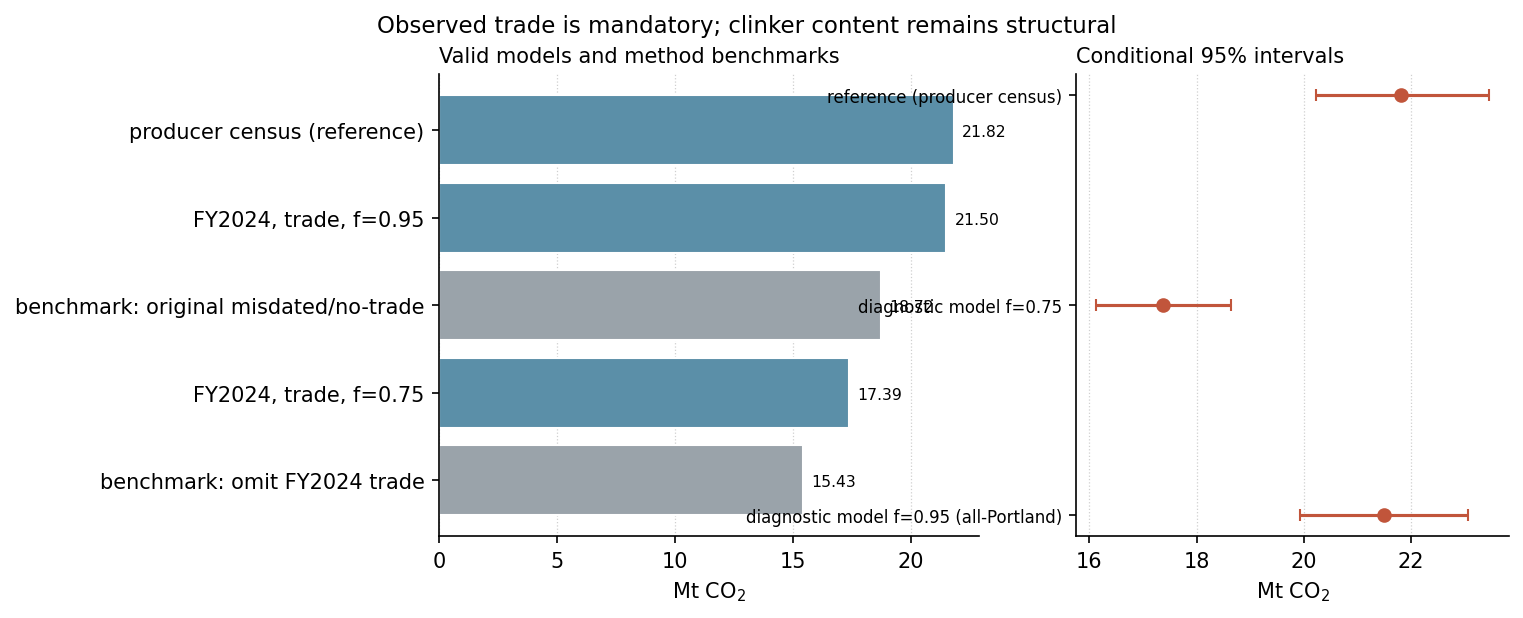
\includegraphics[width=0.98\textwidth]{ippu_cement_evidence.png}
\caption{Left: valid trade-corrected clinker-fraction models and separate method benchmarks.
Right: conditional parametric intervals within the two valid configurations.}
\label{fig:cementevidence}
\end{figure*}

\subsection{Calendar-2022 reconstruction sharpens the official comparison}

The 12 monthly QIM observations sum to \SI{44.331}{\mega\tonne} in calendar 2022. Combining
them with \SI{1.341580}{\mega\tonne} of clinker exports and
\SI{0.003999}{\mega\tonne} of imports gives \SI{34.585831}{\mega\tonne} of inferred clinker
and \SI{17.984632}{\mega\tonne} \COtwo{} at the 0.75 fraction. The 0.95 configuration gives
\SI{22.595056}{\mega\tonne}.

Pakistan's CRT cement row reports \SI{50.2455}{\mega\tonne} of activity and an implied factor
of 0.55539 t/t, yielding \SI{27.905848}{\mega\tonne} \COtwo{}. The independent matched-year
reconstructions are therefore 35.6\% and 19.0\% below the official result. The gap reflects
both activity (44.331 versus 50.246 Mt) and clinker/factor treatment; it is no longer an
artefact of comparing different years.

The CRT reports \SI{49.11203}{\mega\tonne} \COe{} for all IPPU in 2022. Mineral industries
account for 29.300 Mt and chemical industries 19.400 Mt; non-energy products and other
industrial processes contribute 0.217 and 0.192 Mt. All seven numeric background calculations
reproduce exactly, including the ammonia recovery term. The official discrepancy is therefore
methodological and empirical rather than spreadsheet arithmetic.

\begin{figure*}[htbp]
\centering
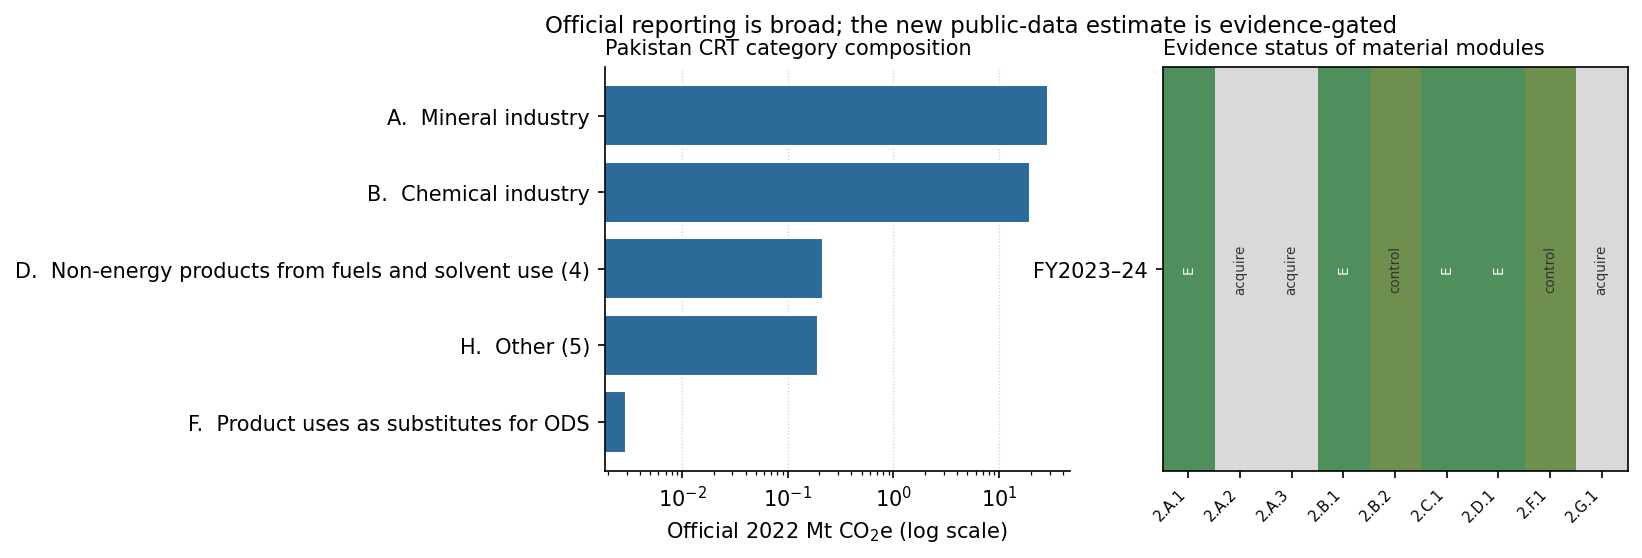
\includegraphics[width=0.92\textwidth]{ippu_official_audit.png}
\caption{Official 2022 IPPU category composition (left) and independent FY2023--24 evidence
status (right). Cement, ammonia, iron and steel and lubricant use are estimated; unsupported rows remain NE.}
\label{fig:official}
\end{figure*}

\subsection{Evidence available for the next categories}

Cement, ammonia, iron and steel, and lubricant use enter the FY2023--24 GHG module. Cement contributes \SI{21.816}{\mega\tonne} CO$_2$ to the \SI{25.535}{\mega\tonne} module total; the following plant evidence identifies remaining process and Tier~2 gaps rather than implying ammonia is wholly absent. One ammonia plant reports
\SI{0.311242}{\mega\tonne} of output in 2024, and historical plant and CDM records identify
nitric-acid technology and abatement projects. National estimates require complete plant
coverage, recovered \COtwo{} and annual abatement operation. For ammonia the generated
reconciliation now compares four independent activity pathways and locates the
inconsistency: the official 2022 filing's \SI{11467}{\kilo\tonne} of ammonia would require
roughly half again more gas than the whole fertiliser sector draws, embodied ammonia in
NFDC's product-wise production sits near \SI{4500}{\kilo\tonne}, and the quantifiable plant
floor is \SI{548}{\kilo\tonne} from two of eight census plants. The filing's recovery term,
by contrast, implies \SI{6442}{\kilo\tonne} of urea, consistent with audited production;
the suspect leg is the activity, not the recovery. The HFC evidence similarly
requires species- and application-specific equipment data before consumption can be related to
annual emissions.

Chemical observations are reported separately by year, and verified CDM reductions are
assigned only to their stated monitoring periods. For Pakarab, the available evidence includes
line-level production, operating days and abatement technology for 2008.

Cement has the most detailed company-level production support. Ammonia retains product-derived output and recovery assumptions; nitric acid still lacks complete own-year production and demonstrated abatement operation. The primary geographic product preserves company-level uncertainty and licence-compatible locations, with unsupported placement retained in the unallocated account.

\subsection{Air-pollutant process coverage}
The admitted air classes estimate ammonia-process releases, electric-route steel emissions and soda-ash process emissions with their specific factors and physical activities. Cement air factors cover an integrated kiln stack and are accounted once under industry; cement GHG calcination remains separate from kiln fuel. Urea finishing, nitric-acid pollutants, lime, glass and other unresolved processes remain explicit coverage gaps. Missing species are not filled with zero or with an uncontrolled screening endpoint.
